% Fonte editável de fig/spea2_aptidao_pt.pdf (Figura da atribuição de aptidão
% e da truncagem do SPEA2, Cap. 2, Seção 2.1). Esquemática: os pontos são
% ilustrativos e não vêm de nenhuma execução. Os valores foram calculados com a
% mesma regra de src/matlab/lib/PlatEMO/Algorithms/Multi-objective
% optimization/SPEA2/{CalFitness,EnvironmentalSelection}.m sobre as 14
% soluções abaixo, tomadas como a união população + arquivo:
%   k = floor(sqrt(14)) = 3; D = 1/(sigma_k + 2), sigma_k sobre a união.
% Rótulo  (f1, f2)          S  R  sigma_k  F
% E1      (0,020; 0,8886)   2  0  0,244    0,4456
% C1      (0,120; 0,6656)   2  0  0,208    0,4528
% C2      (0,165; 0,6058)   1  0  0,134    0,4687
% C3      (0,210; 0,5517)   1  0  0,125    0,4705  <- maior F entre as não dominadas
% C4      (0,255; 0,5070)   1  0  0,134    0,4687
% C5      (0,300; 0,4643)   1  0  0,196    0,4555
% I       (0,580; 0,3284)   0  0  0,344    0,4267  <- menor F entre as não dominadas
% E2      (0,840; 0,1035)   2  0  0,152    0,4646
% F2      (0,950; 0,0403)   1  0  0,210    0,4525
% D1      (0,060; 0,9700)   0  2  dominada por E1
% D1b     (0,130; 0,9300)   0  4  dominada por E1 e C1
% D2      (0,860; 0,2300)   0  2  dominada por E2
% D2b     (0,990; 0,1300)   0  3  dominada por E2 e F2
% D3      (0,360; 0,7000)   0  6  dominada por C1, C2, C3, C4 e C5
% Os três vizinhos mais próximos de I são D2 (0,297), C5 (0,311) e E2 (0,344);
% os de C3 são C4 (0,063), C2 (0,070) e C5 (0,125). Com 9 não dominadas e
% 7 vagas, a truncagem remove C4 e depois C2. Fronteira f2 = 1 - sqrt(f1);
% distância de I à fronteira 0,075, das demais não dominadas no máximo 0,018.
% Os eixos têm a mesma escala, de modo que os círculos são círculos em objetivos.
%
% Regenerar, a partir de thesis/masters/ (a primeira compilação baixa o TikZ;
% o build da dissertação só inclui o PDF e continua offline):
%   tectonic -o fig fig/src/spea2_aptidao_pt.tex
\documentclass[border=2pt]{standalone}
\usepackage{fontspec}
\setmainfont{texgyreheros}[
  Extension = .otf,
  UprightFont = *-regular,
  BoldFont = *-bold,
]
\usepackage{tikz}
\usetikzlibrary{arrows.meta}

% Coordenadas nomeadas (ver tabela acima).
\newcommand{\coordenadas}{%
  \coordinate (E1) at (0.020,0.8886);
  \coordinate (C1) at (0.120,0.6656);
  \coordinate (C2) at (0.165,0.6058);
  \coordinate (C3) at (0.210,0.5517);
  \coordinate (C4) at (0.255,0.5070);
  \coordinate (C5) at (0.300,0.4643);
  \coordinate (I)  at (0.580,0.3284);
  \coordinate (E2) at (0.840,0.1035);
  \coordinate (F2) at (0.950,0.0403);
  \coordinate (D1) at (0.060,0.9700);
  \coordinate (D1b) at (0.130,0.9300);
  \coordinate (D2) at (0.860,0.2300);
  \coordinate (D2b) at (0.990,0.1300);
  \coordinate (D3) at (0.360,0.7000);
}
\def\naodominadas{E1,C1,C2,C3,C4,C5,I,E2,F2}
\def\dominadas{D1,D1b,D2,D2b,D3}

\tikzset{
  nd/.style={circle, draw=black, fill=black, inner sep=0pt, minimum size=4.6pt},
  dom/.style={circle, draw=black!70, fill=white, line width=0.6pt, inner sep=0pt, minimum size=4.4pt},
  xis/.style={black, line width=1.1pt},
  fronteira/.style={black!25, line width=0.8pt},
  dominancia/.style={-{Latex[length=1.3mm]}, black!55, line width=0.45pt, shorten <=2.6pt, shorten >=2.8pt},
  vizinho/.style={black!70, line width=0.55pt, dash pattern=on 2pt off 1.3pt},
  raio/.style={black!70, line width=0.45pt},
  titulo/.style={anchor=south west, font=\bfseries, inner sep=0pt},
  num/.style={font=\fontsize{7}{8}\selectfont, inner sep=2pt},
  nota/.style={font=\fontsize{7.5}{9}\selectfont, inner sep=1pt, align=left},
}

\newcommand{\eixos}{%
  \draw[fronteira] plot[domain=0:1, samples=80, smooth] (\x, {1 - sqrt(\x)});
  \draw[-{Latex[length=1.8mm]}, line width=0.6pt] (0,0) -- (1.1,0) node[below, inner sep=2pt] {$f_1$};
  \draw[-{Latex[length=1.8mm]}, line width=0.6pt] (0,0) -- (0,1.06) node[left, inner sep=2pt] {$f_2$};
}

% \xis{coordenada}: marca de remoção sobre um ponto
\newcommand{\marcaxis}[1]{%
  \draw[xis] ($(#1)+(-0.032,-0.032)$) -- ($(#1)+(0.032,0.032)$);
  \draw[xis] ($(#1)+(-0.032,0.032)$) -- ($(#1)+(0.032,-0.032)$);
}
\usetikzlibrary{calc}

\begin{document}
\fontsize{8}{10}\selectfont
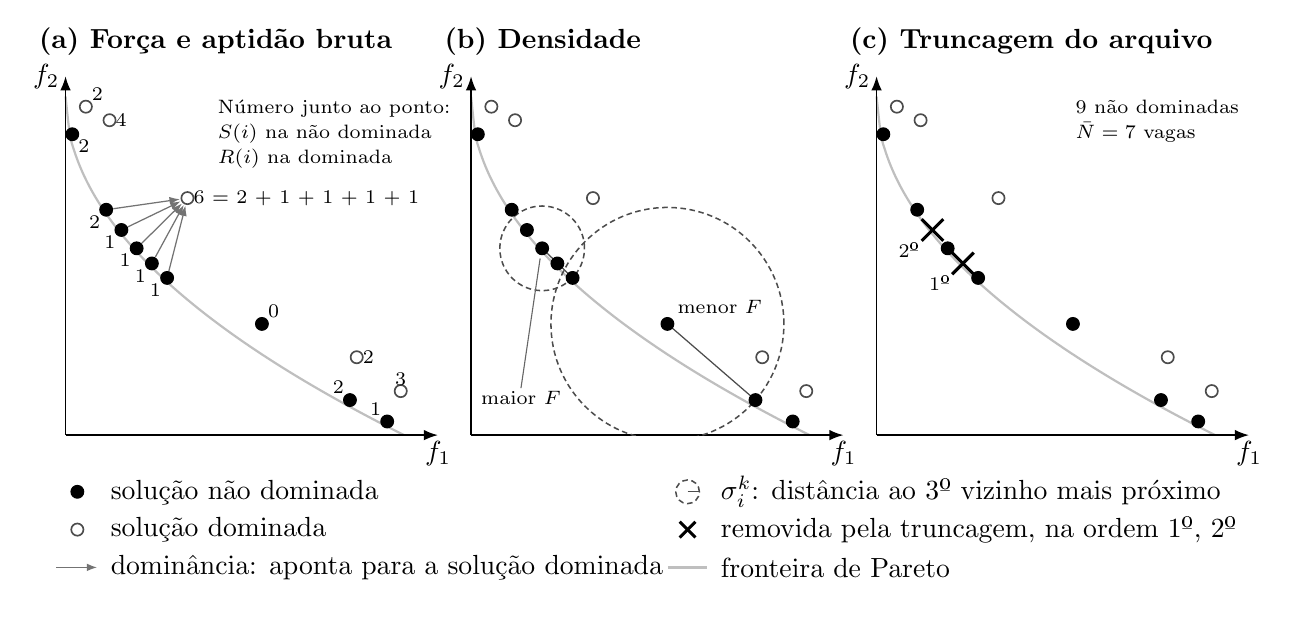
\begin{tikzpicture}[x=4.3cm, y=4.3cm]

  % ---------------- (a) força e aptidão bruta ----------------
  \begin{scope}
    \coordenadas
    \eixos
    \node[titulo] at (-0.08,1.12) {(a) Força e aptidão bruta};
    \foreach \p in {C1,C2,C3,C4,C5} { \draw[dominancia] (\p) -- (D3); }
    \foreach \p in \dominadas { \node[dom] at (\p) {}; }
    \foreach \p in \naodominadas { \node[nd] at (\p) {}; }
    % força S(i) das não dominadas
    \node[num, anchor=north west] at (E1) {2};
    \node[num, anchor=north east] at (C1) {2};
    \node[num, anchor=north east] at (C2) {1};
    \node[num, anchor=north east] at (C3) {1};
    \node[num, anchor=north east] at (C4) {1};
    \node[num, anchor=north east] at (C5) {1};
    \node[num, anchor=south west] at (I) {0};
    \node[num, anchor=south east] at (E2) {2};
    \node[num, anchor=south east] at (F2) {1};
    % aptidão bruta R(i) das dominadas
    \node[num, anchor=south west] at (D1) {2};
    \node[num, anchor=west] at (D1b) {4};
    \node[num, anchor=west] at (D2) {2};
    \node[num, anchor=south] at (D2b) {3};
    \node[num, anchor=west] at (D3) {6 = 2 + 1 + 1 + 1 + 1};
    \node[nota, anchor=north west] at (0.44,1.0) {Número junto ao ponto:\\$S(i)$ na não dominada\\$R(i)$ na dominada};
  \end{scope}

  % ---------------- (b) densidade ----------------
  \begin{scope}[xshift=5.15cm]
    \coordenadas
    \eixos
    \node[titulo] at (-0.08,1.12) {(b) Densidade};
    \begin{scope}
      \clip (0,0) rectangle (1.1,1.06);
      \draw[vizinho] (I) circle (0.344);
      \draw[vizinho] (C3) circle (0.125);
    \end{scope}
    \draw[raio] (I) -- (E2);
    \draw[raio] (C3) -- (C5);
    \foreach \p in \dominadas { \node[dom] at (\p) {}; }
    \foreach \p in \naodominadas { \node[nd] at (\p) {}; }
    \node[nota, anchor=south west] at ($(I)+(0.02,0.02)$) {menor $F$};
    \node[nota, anchor=south west] (maiorF) at (0.02,0.08) {maior $F$};
    \draw[black!60, line width=0.4pt] (maiorF.north) -- ($(C3)+(-0.006,-0.03)$);
  \end{scope}

  % ---------------- (c) truncagem ----------------
  \begin{scope}[xshift=10.3cm]
    \coordenadas
    \eixos
    \node[titulo] at (-0.08,1.12) {(c) Truncagem do arquivo};
    \foreach \p in \dominadas { \node[dom] at (\p) {}; }
    \foreach \p in {E1,C1,C3,C5,I,E2,F2} { \node[nd] at (\p) {}; }
    \marcaxis{C4}
    \marcaxis{C2}
    \node[num, anchor=north east] at ($(C4)+(-0.02,-0.02)$) {1º};
    \node[num, anchor=north east] at ($(C2)+(-0.02,-0.02)$) {2º};
    \node[nota, anchor=north east] at (1.08,1.0) {9 não dominadas\\$\bar{N} = 7$ vagas};
  \end{scope}

  % ---------------- legenda ----------------
  \begin{scope}[x=1cm, y=1cm, shift={(0,-0.72)}]
    \def\lin{0.48}
    \node[nd] at (0.15,0) {};          \node[anchor=west] at (0.45,0) {solução não dominada};
    \node[dom] at (0.15,-\lin) {};     \node[anchor=west] at (0.45,-\lin) {solução dominada};
    \draw[dominancia, shorten <=0pt, shorten >=0pt] (-0.12,-2*\lin) -- (0.4,-2*\lin);
                                       \node[anchor=west] at (0.45,-2*\lin) {dominância: aponta para a solução dominada};
    \draw[vizinho] (7.9,0) circle (0.15); \draw[raio] (7.9,0) -- (8.05,0);
                                       \node[anchor=west] at (8.2,0) {$\sigma_i^k$: distância ao 3º vizinho mais próximo};
    \draw[xis] (7.8,-\lin-0.1) -- (8.0,-\lin+0.1); \draw[xis] (7.8,-\lin+0.1) -- (8.0,-\lin-0.1);
                                       \node[anchor=west] at (8.2,-\lin) {removida pela truncagem, na ordem 1º, 2º};
    \draw[fronteira] (7.65,-2*\lin) -- (8.15,-2*\lin);
                                       \node[anchor=west] at (8.2,-2*\lin) {fronteira de Pareto};
  \end{scope}
\end{tikzpicture}
\end{document}
